\documentclass[12pt,titlepage]{report}
\usepackage[russian]{babel}
\usepackage{amsmath}
\usepackage{amsthm}
\usepackage{amssymb}
\usepackage{longtable}
\usepackage[dvips]{graphics,epsfig}
\usepackage{multirow}
\usepackage{rotating}
\usepackage{fancyhdr}
%\usepackage{eskdplain}
\usepackage{xcolor}
\usepackage{array}
\usepackage[utf8]{inputenc}
\usepackage{psfrag}
\graphicspath{{Pictures/}}
\frenchspacing
\usepackage{graphicx}
%\textwidth=16cm
%\textheight=25cm
\usepackage[left=3cm,right=1cm,top=2cm,bottom=3.5cm,bindingoffset=1.25cm]{geometry}
\renewcommand{\baselinestretch}{1.5}
\newcommand{\jj}{\righthyphenmin=20 \justifying}
%\renewcommand{\rmdefault}{ftm}
\topmargin=-1.0in
\oddsidemargin=0mm
\newcommand{\tocsecindent}{\hspace{7mm}}
\newcommand\ds{\displaystyle}
\newtheorem*{prim}{Примечание}
\newtheorem*{opred}{Определение}
\newtheorem{remark}{Замечание}
\newtheorem{theorem}{Теорема}
\newtheorem*{theorem*}{Теорема}
%\newtheorem{theorem}{Теорема}
%\newtheorem*{theorem*}{Теорема}
\newtheorem{definition}{Определение}%[chapter]
\newtheorem*{definition*}{Определение}
%\newtheorem{deff}{Определение}
%\newtheorem*{ddeff}{Определение}
\newtheorem*{corollary*}{Следствие}
\newtheorem*{example*}{Пример}
\newtheorem*{lemma*}{Лемма}
\newtheorem*{remark*}{Замечание}
\newtheorem*{utv*}{Утверждение}
\newtheorem*{ppredlojenie*}{Предложение}
\newtheorem{upr}{Упражнение}
\newtheorem*{upr*}{Упражнение}
\newtheorem{object}{Определение}
\newtheorem{approval}{Утверждение}
\newtheorem*{vvedenie}{Введение}
\newtheorem*{myth}{Теорема}
\newtheorem{example}{Пример}
\newtheorem{lemma}{Лемма}
\newtheorem{task}{Задача}
\newtheorem{sledstvie}{Следствие}
\renewcommand{\thesection}{\arabic{section}.}
%\renewcommand{\arraystretch}
%\def\R{\mathbb R}
\topmargin=-0.5cm
\usepackage{indentfirst} % Красная строка

\topmargin=-0.5cm

\begin{document}
	\pagestyle{plain}
\begin{center}
	\large{\textbf{ФИЛИАЛ МГУ имени М. В. ЛОМОНОСОВА в городе БАКУ\\[1mm]
			ФАКУЛЬТЕТ ПРИКЛАДНОЙ МАТЕМАТИКИ
	}}
\end{center}

\vskip 3.5cm
\begin{center}
	\LARGE{\textbf{КУРСОВАЯ РАБОТА} \\[1cm]}
	\large{\textbf{«О поведении на бесконечности решений в полосе»}\\[0.3cm]}
	\large{\textbf{студента III курса группы № 217}\\[0.3cm]} 
	\large{\textbf{Каляева Тимура Джанбулатовича}\\[2.1cm]}                                          
\end{center}

\begin{flushright} \large{\textbf{Научный руководитель:\\[3mm]
			д.ф.-м.н, профессор\\
			Чечкин Григорий Александрович}}
\end{flushright}

\vfill

\begin{center}
	\large{\textbf{Баку --- 2020}}
\end{center}
\pagestyle{empty}
\clearpage
\pagestyle{plain}
\clearpage
\tableofcontents
\clearpage

\section*{Введение}
\addcontentsline{toc}{section}{Введение}
Густые каскадные соединения являются моделями во многих областях как естественных, так и прикладных наук, например нанотехнологий, микротехники, современной инженерии (микрорадиаторы), многих физических и биологических
систем.

Колебательные системы с концентрированными массами, имеющими диаметр порядка $\mathcal{O}(\varepsilon)$, изучаются достаточно давно. Экспериментально установлено, что наличие масс ведет к изменению главных частот колебаний и локализации колебаний в окрестности концентрированных масс.

\begin{center}
	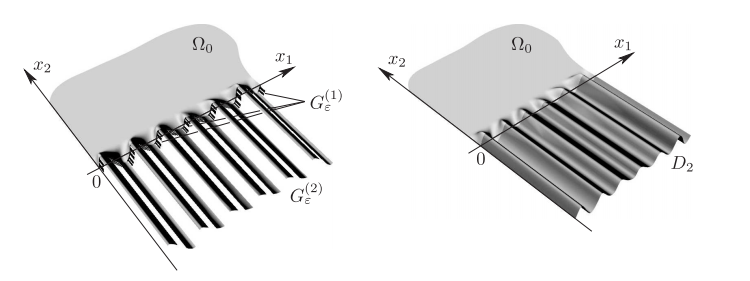
\includegraphics[scale=0.75]{kursac2.png}\\
	Рис.1 Густые каскадные соединения.
\end{center}

В процессе изучения колебаний густых каскадных соединений возникает задача о нахождении коэффиентов уравнения. Каждый коэффицент является решением некой краевой задачи Неймана, при этом не каждое решение имеет ограниченое решение на области. В этой работе мы рассматриваем одну из таких краевых задач. Мы докажем лемму, в которой доказывается условие разрешимости краевой задачи, приведем поставленную задачу к разрешимому случаю и найдем решение, а также его асимптотики.  

В главе 1 рассматривается постановка задачи.  Была определена область\\ $\Pi=\Pi^{-} \cup \Pi^{+} \cup \Pi_{l_{1}}$. Для этой области исследуем краевую задачу (\ref{eq1}) и вводим теорему \ref{teor1} определяющую решение задачи (\ref{eq1}) с данными ассимптотиками. Теорема будет доказана в главе 3.

В главе 2 изучается условие разрешимости, доказанное в лемме (\ref{lem1}), а также свойства решений, описанные в замечаниях (\ref{rem1}) и (\ref{rem2}).

В главе 3 доказывается теорема \ref{teor1}, определяющая разрешимость поставленной задачи (\ref{eq1}).  Её доказательство вытекает из леммы (\ref{lem1}), сформулированной и доказанной в главе 2. Проведя некоторые рассуждения, мы получаем, что решение задачи существует когда $\mu=\frac{4 h_{1} l_{1} \lambda_{0}}{h_{2}}$, и полученное решение определено с точностью до константы, а также симметрично по $\eta_{1}$ относительно $\frac{1}{2}$.
\\
\newpage
\section{Постановка задачи}
Пусть $a, b_{1}, b_{2}, h_{1}, h_{2}$ - положительные действительные числа такие, что:
$$0<b_{1}<b_{2}<\frac{1}{2}, \quad 0<b_{1}-\frac{h_{1}}{2}, \quad b_{1}+\frac{h_{1}}{2}<b_{2}-\frac{h_{1}}{2}, \quad b_{2}+\frac{h_{1}}{2}<\frac{1}{2}-\frac{h_{2}}{2}.$$
Эти неравенства означают,что интервалы
$$\begin{array}{c}
\left(b_{1}-\frac{h_{1}}{2}, b_{1}+\frac{h_{1}}{2}\right), \quad\left(b_{2}-\frac{h_{1}}{2}, b_{2}+\frac{h_{1}}{2}\right), \quad\left(\frac{1-h_{2}}{2}, \frac{1+h_{2}}{2}\right) \\
\left(1-b_{2}-\frac{h_{1}}{2}, 1-b_{2}+\frac{h_{1}}{2}\right), \quad\left(1-b_{1}-\frac{h_{1}}{2}, 1-b_{1}+\frac{h_{1}}{2}\right)
\end{array}$$
содержатся в (0,1) и не пересекаются. \\
Рассмотрим область:
	$$\Pi=\Pi^{-} \cup \Pi^{+} \cup \Pi_{l_{1}}.$$
\begin{center}
		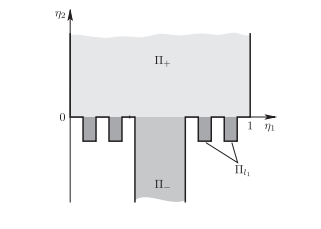
\includegraphics[scale=1.5]{kursac1.png}\\
	Рис.1 Ячейка периодичности.
\end{center}

Здесь: $$\Pi^{+}=(0,1) \times(0,+\infty),$$
$$\Pi^{-}=\left(\frac{1}{2}-\frac{h_{2}}{2}, \frac{1}{2}+\frac{h_{2}}{2}\right) \times(-\infty, 0],$$ $$\Pi_{l_{1}}:=\bigcup_{k=1}^{4} \bar{\Pi}_{k},$$  $$\Pi_{k}=\left(d_{k}-\frac{h_{1}}{2}, d_{k}+\frac{h_{1}}{2}\right) \times\left(-l_{1}, 0\right],$$ \\
где $d_{1}=b_{1}$, $d_{2}=b_{2}$, $d_{3}=1-b_{2}$, $d_{4}=1-b_{1}$.
\\
Рассмотрим следующую краевую задачу на этой области:

\begin{equation}
	\label{eq1}
	\left\{\begin{array}{ll}
		-\Delta_{\eta} Z_{1}^{(0)}(\eta) =\left\{\begin{array}{ll}
			0, & \eta \in \Pi^{+} \cup \Pi^{-}, \\
			\lambda_{0}, & \eta \in \Pi_{l_{1}},
		\end{array}\right. \\
		\partial_{\eta_{1}} Z_{1}^{(0)}(\eta)=0, & \eta \in \partial \Pi_{\|},\\
		\partial_{\eta_{1}}^{s} Z_{1}^{(0)}\left(0, \eta_{2}\right)=\partial_{\eta_{1}}^{s} Z_{1}^{(0)}\left(1, \eta_{2}\right), & \eta_{2}>0, \quad s=0,1,\\
		\partial_{\eta_{2}} Z_{1}^{(0)}\left(\eta_{1}, 0\right)=0, & \left(\eta_{1}, 0\right) \in \partial \Pi, \quad\\ \partial_{\eta_{2}} Z_{1}^{(0)}\left(\eta_{1},-l_{1}\right)=0, & \left(\eta_{1},-l_{1}\right) \in \partial \Pi.
	\end{array}\right.
\end{equation}

\begin{theorem}
	\label{teor1}
	Существует решение $Z_{1}^{(0)} \in H_{\mathrm{loc}, \eta_{2}}^{1}(\Pi)$ задачи (\ref{eq1}) со следующими асимптотиками:
	
	\begin{equation}
	\label{eq2}
		Z_{1}^{(0)}(\eta)=\left\{\begin{array}{ll}
		C_{1}^{(0)}+\mathcal{O}\left(\exp \left(-2 \pi \eta_{2}\right)\right), & \eta_{2} \rightarrow+\infty, \\
		\frac{4 h_{1} l_{1} \lambda_{0}}{h_{2}} \eta_{2}-\frac{C_{1}^{(0)}}{h_{2}}+\mathcal{O}\left(\exp \left(\pi h_{2}^{-1} \eta_{2}\right)\right), & \eta_{2} \rightarrow-\infty.
		\end{array}\right.
	\end{equation}\\
	Более того, функция $Z_{1}^{(0)}$ является четной по $\eta_{1}$ относительно $\frac{1}{2}$.
\end{theorem}

\newpage
\section{Вспомогательные утверждения}
Изучим некоторые свойства следующей краевой задачи
\begin{equation}
\label{eq3}
	\left\{\begin{array}{ll}
		-\Delta_{\eta} Z(\eta)=F(\eta), & \eta \in \Pi, \\
	\partial_{\eta_{1}} Z(\eta) =B(\eta), & \eta \in \partial \Pi_{\|}, \eta_{2}<0, \\
	\partial_{\eta_{2}} Z\left(\eta_{1}, 0\right)=0, & \left(\eta_1, 0\right) \in \partial \Pi,\\
	\left.\partial_{\eta_{1}}^{k} Z(\eta)\right|_{\eta_{1}=0} =\left.\partial_{\eta_{1}}^{k} Z(\eta)\right|_{\eta_{1}=1}, & \eta_{2}>0 ; k=0,1.
	\end{array}\right.
\end{equation}

Для начала изучим разрешимость этой задачи. Пусть $\widehat{C}_{0}^{\infty}(\bar{\Pi})$ пространтво бесконечно дифференцируемых функций в $\bar{\Pi}$, которые удовлетворяют периодическим условиям $\left.\partial_{\eta_{1}}^{k} Z(\eta)\right|_{\eta_{1}=0} =\left.\partial_{\eta_{1}}^{k} Z(\eta)\right|_{\eta_{1}=1}$, $\eta_{2}>0$; $k=0,1$ и ограничены по $\eta_{2}$:

$$\forall v \in \widehat{C}_{0}^{\infty}(\bar{\Pi}) \; \exists R>0 \; \forall \eta \in \bar{\Pi}\left|\eta_{2}\right| \geq R: \quad v(\eta)=0.$$\\
Пусть $\mathcal{H}$ будет замыканием пространства $\widehat{C}_{0}^{\infty}(\bar{\Pi})$ по норме 
$$\|u\|_{\mathcal{H}}=\left(\left\|\nabla_{\eta} u\right\|_{L_{2}(\Pi)}^{2}+\|\rho u\|_{L_{2}(\Pi)}^{2}\right)^{\frac{1}{2}},$$\\
где $\rho\left(\eta_{3}\right)=\frac{1}{1+\left|\eta_{2}\right|} \quad\left(\eta_{2} \in \mathbb{R}\right)$. Будем называть функцию $Z$ обощенным решением задачи (\ref{eq3}), если для любой функции $v \in \mathcal{H}$ выполняется интегральное равенство \\
$$\int_{\Pi} \nabla_{\eta} Z \cdot \nabla_{\eta} v d \eta=\int_{\Pi} F v d \eta+\int_{\partial \Pi_{\|}} B v d \eta.$$


\begin{lemma}
	\label{lem1}
	Пусть $_{\rho}^{1} F \in L_{2}(\Pi)$ и $\frac{1}{\rho} B \in L_{2}\left(\partial \Pi_{\|}\right)$, и пусть\\
	\begin{equation}
	\label{eq4}
		\int_{\Pi} F(\eta) d \eta+\int_{\partial \Pi_{\|}} B(\eta) d \sigma_{\eta}=0.
	\end{equation}\\
	Тогда существует решение $Z \in \mathcal{H}$ задачи (\ref{eq3}), которое определено с точностью до константы.
\end{lemma}

\begin{proof}
  	Перепишем уравнение (\ref{eq4}) в виде\\
  	\begin{equation}
	 \label{eq5} 	
	  	\langle Z, v\rangle-\int_{\Pi_{-2,2}} Z v d \eta=\int_{\Pi} F v d \eta+\int_{\partial \Pi_{\|}} B v d \eta,
	 \end{equation}\\
	 где\\
	 $$\Pi_{\alpha, \beta}=\left\{\eta \in \Pi: \alpha<\eta_{2}<\beta\right\}$$\\
	 и\\
	 \begin{equation}
	 \label{eq6}
	 	\langle u, v\rangle=\int_{\Pi} \nabla_{\eta} u \cdot \nabla_{\eta} v d \eta+\int_{\Pi_{-2,2}} u v d \eta.
	 \end{equation}\\
	 
	 Тогда новое скалярное произедение (\ref{eq6}) порождает эквивалентную норму в $\mathcal{H}$. Очевидно, что $\langle u, u\rangle \leq c_{1}\|u\|_{\mathcal{H}}^{2} \quad(u \in \mathcal{H})$. Обратное неравенство с другой константой вытекает из неравенства Харди\\
	 $$\int_{0}^{+\infty} \frac{\phi^{2}\left(\eta_{2}\right)}{\left(1+\eta_{2}\right)^{2}} d \eta_{2} \leq 4 \int_{0}^{+\infty}\left|\partial_{\eta_{2}} \phi\right|^{2} d \eta_{2} \quad\left(\phi \in C^{1}([0,+\infty)) \quad \text { with } \quad \phi(0)=0\right)$$\\
	 и неравенства\\
	 \begin{equation}
	 \label{eq7}
	 \begin{array}{l}
		 \int_{\Pi} \rho^{2}\left(\eta_{2}\right) u^{2}(\eta) d \eta \\
		 \quad \leq \int_{\Pi_{-2,2}} \rho^{2} u^{2} d \eta+\int_{\Pi} \rho^{2}\left(\left(1-\chi\left(\eta_{2}\right)\right) u\right)^{2} d \eta \\
		 \quad \leq \int_{\Pi_{-2,2}} \rho^{2} u^{2} d \eta+c_{\chi}\left(\int_{\Pi}\left(\partial_{\eta_{2}} u\right)^{2} d \eta+\int_{\Pi_{-2,2}}\left(\chi^{\prime}\left(\eta_{2}\right) u\right)^{2} d \eta\right) \\
		 \quad \leq c_{2}\langle u, u\rangle,
		 \end{array}
	 \end{equation}\\
	 где $\chi \in C^{\infty}(\mathbb{R})$, $0 \leq \chi \leq 1$ и
	 \begin{equation}
	 \label{eq8}
		 \chi\left(\eta_{2}\right)=\left\{\begin{array}{ll}
		 1 & \text { if }\left|\eta_{2}\right| \leq 1 \\
		 0 & \text { if }\left|\eta_{2}\right| \geq 2.
		 \end{array}\right.
	 \end{equation}\\
	 В силу условий леммы (\ref{lem1}), неравенства (\ref{eq7}) и неравенства \\
	 \begin{equation}
	 \label{eq9}
	 	\begin{aligned}
		 \int_{\partial \Pi_{\|}} \rho^{2}\left(\eta_{2}\right) v^{2}(\eta) d \sigma_{\eta} & \leq \int_{-\infty}^{0} \rho\left(\eta_{2}\right) \int_{\partial \omega} v^{2} d \sigma_{\eta_{1}} d \eta_{2} \\
		 & \leq c \int_{\Pi}\left(\left|\nabla_{\eta} v\right|^{2}+\rho\left(\eta_{2}\right) v^{2}\right) d \eta
		 \end{aligned} \quad(v \in \mathcal{H})
	 \end{equation}\\
	 правая сторона уравнения (\ref{eq5}) определяет линейный непрерывный функционал из $\mathcal{H}$. Так как вложение $\mathcal{H} \subset L_{2}\left(\Pi_{-2,2}\right)$ компактно, существует самосопряженный положительный компктный оператор $\mathcal{A}: \mathcal{H} \mapsto \mathcal{H}$ такой, что\\
	 $$\langle\mathcal{A} u, v\rangle=\int_{\Pi_{-2,2}} u(\eta) v(\eta) d \eta \quad(\{u, v\} \in \mathcal{H}.$$\\
	 
	 Таким образом, мы можем переписать выражение (\ref{eq5}) в виде\\
	 $$Z-\mathcal{A} Z=f$$\\
	 и применить к нему теоремы Фредгольма. Очевидно, что все решения однородной задачи (\ref{eq3}) является константами (интеграл Дирихле тривиален). Таким образом, получаем, что равенство (\ref{eq4}) является условием разрешимости задачи (\ref{eq3}).\\
	\end{proof}
	 
	 \begin{remark}
	 	\label{rem1}
	 	Пусть $\exp \left(\delta_{0}\left|\eta_{2}\right|\right) F \in L_{2}(\Pi)$ и $\exp \left(-\delta_{0} \eta_{2}\right) B \in L_{2}\left(\partial \Pi_{\|}\right)\left(\delta_{0}>0\right)$. Учитывая характеристики решений эллептических задач в полупрямоугольниках мы можем подобрать решение задачи $\widetilde{Z}$ такое, что\\
	 	$$\exp \left(-\delta_{1} \eta_{2}\right) \widetilde{Z} \in H^{1}\left(\Pi^{-}\right),$$\\
	 	где $\delta_{1}$ это случайное число, которое удовлетворяет неравенствам $0<\delta_{1}<\delta_{0}$ и $\delta_{1}<\sqrt{\Lambda(\omega)}$. Тут $\Lambda(\omega)$ это первое положительное собственное значение задачи Неймана на $\omega = \left(\frac{1}{2}-\frac{h_{2}}{2}, \frac{1}{2}+\frac{h_{2}}{2}\right)$. Очевидно, что решение $\widetilde{Z}$ имеет следующие асимптотики на полупрямоугольнике $\Pi^{+}$:\\
	 	\begin{equation}
	 	\label{eq10}
		 	\tilde{Z}(\eta)=C+O\left(\exp \left(-\delta_{2} \eta_{2}\right)\right) \quad\left(\eta_{2} \rightarrow+\infty\right).
	 	\end{equation}
	\end{remark}
	 
	\begin{remark}
		\label{rem2}
		Если функции $F$ и $B$ из замечания (\ref{rem1}) четные или нечетные по переменной $\eta_{1}$ относительно $\frac{1}{2}$, то и решение $\widetilde{Z}$ имеет ту же симметрию. Например, если \\
		$$F\left(\eta_{1}, \eta_{2}\right)=F\left(1-\eta_{1}, \eta_{2}\right) \quad \text {и} \quad B\left(\eta_{1}, \eta_{2}\right)=B\left(1-\eta_{1}, \eta_{2}\right),$$
		то в силу симметрии $\left(\frac{1}{2}-\frac{h_{2}}{2}, \frac{1}{2}+\frac{h_{2}}{2}\right)$ и использования замены $\eta_{1}=1-\eta_{1}^{\prime}$ в задаче (\ref{eq3}) мы получаем, что разность $\tilde{Z}\left(\eta_{1}, \eta_{2}\right)-\widetilde{Z}\left(1-\eta_{1}, \eta_{2}\right)$ является решением однородной задачи (\ref{eq3}) и представление (\ref{eq10}) удовлетворяет ему. В силу единственности такого решения разность зануляется.
	\end{remark}

\newpage
\section{Доказательство теоремы}

\begin{proof}
	Покажем, что исходная задача (\ref{eq1}) не удовлетворяет условию разрешимости и, следовательно, не имеет ограниченного решения на области $\Pi$:\\
	  $$\int_{\Pi_{l_{1}}} \lambda_{0} d \eta = 4 h_{1} l_{1} \lambda_{0} \neq 0.$$
	Тогда будем искать решение для задачи (\ref{eq1}) в виде \\
	$$Z_{1}^{(0)}(\eta)=\mu \eta_{2} \chi_{-}\left(\eta_{2}\right)+\widetilde{Z}_{1}^{(0)}(\eta), \quad \eta \in \Pi,$$\\
	где $\chi_{-}\left(\eta_{2}\right)$ это сглаживающий оператор, такой что $0 \leq \chi_{-}\left(\eta_{2}\right) \leq 1$; он равен 0, если $\eta_{2} \geq-1$ и равен 1, если $\eta_{2} \leq-2$. Легко видеть, что $\widetilde{Z}_{1}^{(0)}(\eta)$ удовлетворяет следующей краевой задаче:
	\begin{equation}
	\label{eq11}
	\left\{\begin{array}{ll}
	-\Delta_{\eta} \widetilde{Z}_{1}^{(0)}(\eta)=\left\{\begin{array}{ll}
	0, & \eta \in \Pi^{+}, \\
	\mu\left(\eta_{2} \chi_{-}^{\prime \prime}\left(\eta_{2}\right)+2 \chi_{-}^{\prime}\left(\eta_{2}\right)\right), & \eta \in \Pi^{-},\\
	\lambda_{0}, & \eta \in \Pi_{l_{1}},
	\end{array}\right. \\
	\partial_{\eta_{1}}^{s} \tilde{Z}_{1}^{(0)}\left(0, \eta_{2}\right)=\partial_{\eta_{1}}^{s} \tilde{Z}_{1}^{(0)}\left(1, \eta_{2}\right), & \eta_{2}>0, \quad s=0,1,\\
	\partial_{\eta_{2}} \widetilde{Z}_{1}^{(0)}\left(\eta_{1}, 0\right)=0, & \left(\eta_{1}, 0\right) \in \partial \Pi,\\
	\partial_{\eta_{1}} \widetilde{Z}_{1}^{(0)}(\eta)=0, & \eta \in \partial \Pi_{\|}, \eta_{2}<0, \\
	\partial_{\eta_{2}} \widetilde{Z}_{1}^{(0)}\left(\eta_{1},-l_{1}\right) = 0, & \left(\eta_{1},-l_{1}\right) \in \partial \Pi.
	\end{array}\right.
	\end{equation}
	
	Из докзанной ранее леммы (\ref{lem1}) в главе 2 следует, что существует решение задачи (\ref{eq3}) тогда и только тогда, когда
	$$\int_{\Pi^{-}} \mu \left(\eta_{2} \chi_{-}^{\prime \prime}\left(\eta_{2}\right)+2 \chi_{-}^{\prime}\left(\eta_{2}\right)\right) d \eta + \int_{\Pi_{l_{1}}} \lambda_{0} d \eta = 0,$$\\
	и тогда
	$$\mu= \frac{-\int_{\Pi_{l_{1}}} \lambda_{0} d \eta}{\int_{\Pi^{-}} \eta_{2} \chi_{-}^{\prime \prime}\left(\eta_{2}\right)+2 \chi_{-}^{\prime}\left(\eta_{2}\right) d \eta} =\frac{4 h_{1} l_{1} \lambda_{0}}{h_{2}}.$$ \\
	Более того, это решение определено с точностью до константы. Подбирая должным образом эту константу (по замечанию (\ref{rem1})), получаем асимптотики (\ref{eq2}).\\
	Так как правая часть уравнения и краевых условий задачи (\ref{eq11}) четные по переменной $\eta_{1}$ относительно $\frac{1}{2}$, решение $\widetilde{Z}_{1}^{(0)}$ также будет иметь ту же четность в силу замечания (\ref{rem2}). 
\end{proof}





\newpage
\section*{Заключение}
\addcontentsline{toc}{section}{Заключение}
В данной работе была рассмотрена краевая задача Неймана для ячейки переодичности густого каскадного соединения.  Для получения решения поставленной задачи (\ref{eq1}), была сформулирована теорма \ref{teor1}, доказательство которой было главной целью данной задачи. Мы ввели вспогательные утверждения и лемму (\ref{lem1}), из которых и следовало доказательство нашей главной теоремы, показанное в главе 3.

\newpage
\addcontentsline{toc}{section}{Литература}
\begin{thebibliography}
	{1}
	\bibitem{book1}
	\emph {T.A. Mel'nyk} Homogenization of the Poisson equation in a thick periodic junction, Zeitsch. Anal. Anwend. $18(4)(1999),$ pp. $953-975$.
	\bibitem{book2}
	\emph { G.A. Chechkin, T.A. Mel'nyk} "Asymptotics of eigenelements to spectral problem in thick cascade junction with concentrated masses", Appl. Anal.$, \mathbf{9 1 : 6}(2012)$ $1055-1095$.
\end{thebibliography}

\end{document}